\documentclass[border=2pt]{standalone}
\usepackage{mathptmx}\usepackage[scaled=0.92]{helvet}
\usepackage{xcolor}
\usepackage{tikz}
\usetikzlibrary{arrows.meta,positioning,fit,calc}
\usepackage{pgfplots}
\pgfplotsset{compat=1.17}
\definecolor{mapis}{RGB}{164,18,63}
\definecolor{slgray}{RGB}{138,148,156}
\begin{document}
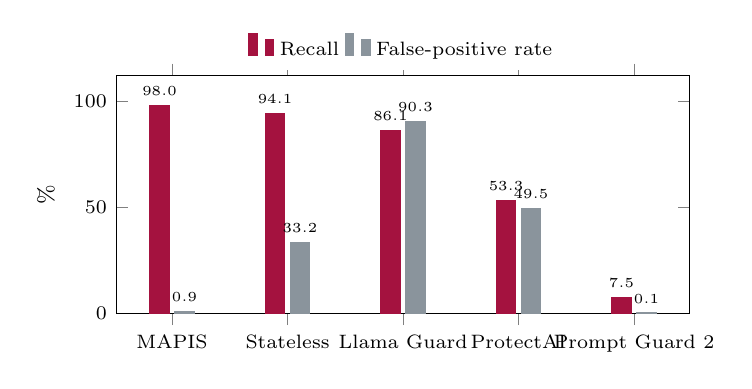
\begin{tikzpicture}
\begin{axis}[ybar, bar width=7pt, width=252pt, height=4.6cm, ymin=0, ymax=112, ylabel={\%}, ylabel style={font=\footnotesize},
 symbolic x coords={MAPIS,Stateless,Llama Guard,ProtectAI,Prompt Guard 2}, xtick=data, x tick label style={font=\scriptsize},
 y tick label style={font=\scriptsize}, legend style={at={(0.5,1.02)},anchor=south,legend columns=2,font=\scriptsize,draw=none},
 nodes near coords={\pgfmathprintnumber[fixed,precision=1,fixed zerofill]{\pgfplotspointmeta}}, nodes near coords style={font=\tiny}, enlarge x limits=0.12]
\addplot[fill=mapis, draw=mapis] coordinates {(MAPIS,98.0) (Stateless,94.1) (Llama Guard,86.1) (ProtectAI,53.3) (Prompt Guard 2,7.5)};
\addplot[fill=slgray, draw=slgray] coordinates {(MAPIS,0.9) (Stateless,33.2) (Llama Guard,90.3) (ProtectAI,49.5) (Prompt Guard 2,0.1)};
\legend{Recall, False-positive rate}
\end{axis}
\end{tikzpicture}
\end{document}
